\documentclass[10pt,letterpaper]{article}
\usepackage[margin=1in]{geometry}
\usepackage{amsmath,amssymb,amsthm,mathtools}
\usepackage{graphicx}
\usepackage{booktabs}
\usepackage[numbers,sort&compress]{natbib}
\usepackage[hidelinks]{hyperref}
\usepackage{xcolor}
\usepackage{microtype}
\usepackage{caption}
\captionsetup{font=small,labelfont=bf}
\newtheorem{theorem}{Theorem}
\newtheorem{lemma}{Lemma}
\newtheorem{proposition}{Proposition}
\newtheorem{corollary}{Corollary}
\theoremstyle{definition}
\newtheorem{definition}{Definition}
\theoremstyle{remark}
\newtheorem{remark}{Remark}
\newcommand{\SB}{\Sigma^{\mathrm{B}}}
\newcommand{\SW}{\Sigma^{\mathrm{W}}}
\newcommand{\E}{\mathbb{E}}
\newcommand{\Var}{\mathrm{Var}}
\newcommand{\Cov}{\mathrm{Cov}}
\newcommand{\NnucPsy}{289{,}279}
\newcommand{\DpsyRange}{744--1{,}164}
\newcommand{\NdMedRange}{12--28}
\newcommand{\DPone}{1{,}054}
\newcommand{\MedPone}{28}
\newcommand{\DPtwo}{1{,}164}
\newcommand{\MedPtwo}{19}
\newcommand{\DPthree}{744}
\newcommand{\MedPthree}{12}
\newcommand{\PBnullCalls}{19{,}158--31{,}617}
\newcommand{\PBnullTI}{0.34--0.44}
\newcommand{\LCPnullCalls}{4{,}986--12{,}880}
\newcommand{\LCPnullTI}{0.20--0.30}
\newcommand{\XDSnullTI}{0.048--0.050}
\newcommand{\XDSnullTop}{0.047--0.053}
\newcommand{\XDSnullMaxCall}{1}
\newcommand{\PBrepFalse}{3{,}798--12{,}827}
\newcommand{\XDSrepFalse}{0}
\newcommand{\PBgrowA}{1{,}063--1{,}778}
\newcommand{\PBgrowC}{7{,}036--10{,}443}
\newcommand{\LCPgrowB}{0--19}
\newcommand{\XUnullCalls}{12{,}073--19{,}934}
\newcommand{\XDSfreshCalls}{0.0--1.3}
\newcommand{\LPBFDRa}{0.48}
\newcommand{\LLCPFDRa}{0.087}
\newcommand{\LPBFDRb}{0.57}
\newcommand{\LLCPFDRb}{0.135}
\newcommand{\LPBFDRc}{0.66}
\newcommand{\LLCPFDRc}{0.217}
\newcommand{\LXDSFDRrange}{0.042--0.053}
\newcommand{\LXDSpowRange}{0.778--0.999}
\newcommand{\SXDSFDRrange}{0.025--0.049}
\newcommand{\SXDSpowDforty}{0.156}
\newcommand{\SLCPpowDforty}{0.501}
\newcommand{\SeaXDSTI}{0.050}
\newcommand{\SeaXDSTop}{0.043--0.050}
\newcommand{\SeaLCPTop}{0.092--0.099}
\newcommand{\SeaPBcalls}{2{,}714--3{,}714}
\newcommand{\RealXDSfrac}{37--63\%}
\newcommand{\RealXDSrep}{68--82\%}
\newcommand{\RealPBrep}{62--80\%}
\newcommand{\RealPBonly}{10{,}086--14{,}643}
\newcommand{\CouplingSEAAD}{0.046}
\newcommand{\CouplingFrac}{58\%}
\newcommand{\CouplingFracLee}{33\%}
\newcommand{\Rcorrln}{0.155}
\newcommand{\Mcorrln}{0.000}
\newcommand{\PBposFrac}{70--82\%}
\newcommand{\CouplePB}{0.524, 0.605, 0.718}
\newcommand{\CoupleLCP}{0.104, 0.143, 0.191}
\newcommand{\CoupleXDS}{0.059, 0.047, 0.056}
\newcommand{\CoupleXU}{0.060, 0.104, 0.223}
\newcommand{\DCtext}{Cell numbers differ between AD cases and controls in all three PsychAD subtypes (medians 21 versus 36 nuclei in Homeo\_CECR2, 23 versus 18 in PVM\_CD163 and 17 versus 10 in ADAM\_GPNMB; Mann--Whitney $p\le8\times10^{-5}$). By Propositions~\ref{prop:leak} and~\ref{prop:transform}, groups with different cell numbers have different biases, so comparing co-expression between groups should produce false differences. We tested this in the real-cell null, with each pseudo-donor carrying the AD label of the real donor whose cell number it has (three reassignments per subtype; frozen plan DC\_PREREG). Pseudobulk differential co-expression (difference of Fisher-transformed correlations) made 718--5{,}634 false calls per reassignment (per-pair type-I 0.13--0.21), so the pre-registered decision that pseudobulk differential co-expression is confounded by cell number is YES. XDS differential co-expression (Welch test of the per-donor cross-split products between groups) made 0 (type-I 0.048--0.052; decision YES), and the leak-corrected version made 0--6 (type-I 0.048--0.056). On real donors pseudobulk reported 5{,}806, 2{,}441 and 2{,}561 AD-associated co-expression changes in Homeo\_CECR2, PVM\_CD163 and ADAM\_GPNMB. With only cell-number differences it makes 5{,}188, 3{,}134 and 1{,}002 on average, that is 89\%, 128\% and 39\% of those numbers, so in the first two subtypes pseudobulk differential co-expression cannot be distinguished from the cell-number artifact. XDS reported 816, 19 and 0. The caveat of Section~\ref{sec:null} applies: the pooled null has somewhat stronger within-donor structure than real donors.}
\newcommand{\SplitText}{XDS uses one random split per donor. On real PsychAD donors we repeated XDS with three split seeds (post hoc). The numbers of BH calls were Homeo\_CECR2 50{,}210, 49{,}779, 49{,}835; PVM\_CD163 54{,}679, 54{,}794, 54{,}663; ADAM\_GPNMB 33{,}312, 33{,}267, 33{,}302, and the Jaccard index between call sets from different seeds was 0.79 (Homeo\_CECR2); 0.83 (PVM\_CD163); 0.67 (ADAM\_GPNMB). Call counts are stable, but a fifth to a third of individual calls depend on the seed; aggregating several splits (for example by a Cauchy combination of $p$-values) is a natural extension that we have not evaluated.}


\title{Why pseudobulk gene co-expression fails in large single-cell cohorts, and how to fix it}
\author{[Author names and affiliations to be added by the authors]}
\date{}

\begin{document}
\maketitle

\begin{abstract}
Between-donor gene co-expression in single-cell cohorts is usually tested by correlating pseudobulk donor means. We show that this test fails increasingly as cohorts grow: within-donor cell-state covariance leaks into donor means in proportion to each donor's inverse cell count, and log or variance transformations add a factor shared by all genes; each bias is fixed per donor, so their sum grows like the number of donors $D$ while noise grows like $\sqrt D$. In real-cell nulls from 744--1{,}164 PsychAD brain myeloid donors per subtype, pseudobulk called \RfPBmean{} of about 89{,}000 gene pairs per run, and adjusting for cell number and depth, weighting donors or removing principal components left false calls in every run. We propose XDS-M, which measures the two genes of a pair on disjoint random halves of each donor's cells, standardizes by the donor's design only, and averages a studentized cross-product test over five splits; we prove per-pair asymptotic normality. From 100 donors up, XDS-M made a false call in 3--8\% of null runs and met pre-specified bounds in \XDSMholdsLarge{} brain and blood settings; it failed a brain-bank-stratified null in two of three subtypes and passed once bank means were removed. At 25--50 donors only permutation-based XDS was not rejected, with little power. Donor maps show null pseudo-donors ordered by cell count, and a function-text gene map built in the Mantis platform shows pseudobulk's false edges as concentrated within function clusters as real edges, so such coherence does not validate edges. Because Alzheimer's cases and controls differ in cell numbers, pseudobulk also reports false differential co-expression, which a group-centred, unstandardized XDS-M avoids.

\end{abstract}

\section{Introduction}

Single-cell RNA-seq cohorts now profile hundreds to thousands of donors: the PsychAD prefrontal-cortex myeloid atlas profiled 1,607 donors \citep{Lee2023PsychADmyeloid}, and co-expression has been mapped across 982 blood donors of the OneK1K cohort \citep{Zhang2026scpcQTL}. One reason to collect so many donors is to study how genes co-vary \emph{between} donors, through genetic, environmental, disease or technical differences. Between-donor co-expression underlies co-expression QTL mapping \citep{vanderWijst2018,Li2023coeQTL}, donor-level gene networks \citep{Lu2023Dozer} and comparisons of co-expression between cases and controls. It is almost always computed in the same way: average each donor's cells of one type into a pseudobulk profile and correlate the profiles across donors. Pseudobulk is regarded as the safe choice for donor-level inference because it treats the donor, not the cell, as the unit of replication \citep{Squair2021,Zimmerman2021}.

We show that for co-expression this safety is illusory, and that the failure becomes worse as cohorts grow. The reason is simple. A pseudobulk correlation is a sum over donors, and every donor contributes a small bias that does not depend on the number of donors $D$: it depends on the donor's own cell number. The summed bias grows like $D$ while the noise grows like $\sqrt D$, so at population scale the bias dominates. We identify three such per-donor biases (Section~\ref{sec:bias}). First, cell-state programs leak into donor means: the covariance of donor means is the between-donor covariance plus the within-donor covariance scaled by the donor's effective inverse cell count. Second, any transformation of a donor mean whose expectation depends on the donor's cell number, such as log-CPM or standardizing by the donor's own estimated sampling variance, adds a factor shared by all genes. Third, coupling between a cell's sequencing depth and its state biases moment corrections of the first two problems.

These biases defeat not only pseudobulk but also corrections of it. We built a leak-corrected permutation test (LCP) and several refinements of it, and each failed on real cells at population scale in a way the theory predicts (Section~\ref{sec:neg}). What works is to remove the within-donor term by design rather than estimate it: split each donor's cells at random into two halves, take one gene's donor mean from one half and the other gene's from the other half, and standardize each mean using only the donor's design (cell number and depth). We call the resulting donor-permutation test XDS. Its validity requires many donors but not many cells per donor (Theorem~\ref{thm:xds}), which is the regime of population cohorts.

Our evaluation rests on exact nulls built from real cells. Pooling the nuclei of one cell type and reassigning them to pseudo-donors with the real donors' cell numbers yields data with every real within-cell program and every real cell-number imbalance, but with zero between-donor covariance for every gene pair. In \NnucPsy{} PsychAD microglia and perivascular-macrophage nuclei with \DpsyRange{} pseudo-donors per subtype, pseudobulk declares \PBnullCalls{} of roughly 89,000 gene pairs co-expressed, and \PBrepFalse{} of these false edges replicate in an independent half of the pseudo-donors. XDS makes at most one false call. Because cell numbers differ between Alzheimer's disease (AD) cases and controls, the same artifact produces false \emph{differential} co-expression between them (Section~\ref{sec:dc}).

\paragraph{Contributions.} (i) A decomposition of pseudobulk co-expression bias into three per-donor terms, and a result showing that any non-vanishing per-donor bias drives the false-positive rate to one as $D$ grows (Theorem~\ref{thm:growth}). (ii) XDS, a cross-split, design-standardized donor-permutation test, valid as $D\to\infty$ with bounded cells per donor. (iii) Exact real-cell nulls at up to 1,164 donors and simulations up to 1,000 donors, with false discoveries reported as a function of cohort size. (iv) A pre-registered record of six corrections that fail and why. (v) A demonstration that cell-number differences between AD cases and controls create false differential co-expression. All analyses followed plans frozen before they were run; the plans, their hashes and every deviation are listed in Appendix~\ref{app:prereg}.

\paragraph{Related work.} Within-cell co-expression methods model counts given latent expression to remove measurement noise \citep{Su2023CSCORE,Lu2023Dozer}; they target a different estimand from ours. Count splitting and data thinning split each cell's counts into independent folds to avoid double use of data \citep{Neufeld2024countsplit,Neufeld2024thinning,Dharamshi2025gdt}. Thinning removes technical noise shared between folds but not cell state, which both folds of a cell share, so it does not remove the leak; splitting \emph{cells} does. The leak is a count-scale instance of the measurement-error decomposition behind BCES-type estimators \citep{AkritasBershady1996,Kelly2007}, and our design-only variances borrow the Paule--Mandel construction \citep{PauleMandel1982}. Calibration of single-cell analyses with synthetic or knock-off nulls is an active topic at RECOMB \citep{Song2025ClusterDE,Jiang2025Nullstrap}; our nulls instead permute real cells.

\section{Setting}\label{sec:setting}

Donors $d=1,\dots,D$ contribute $n_d$ cells of one type. Cell $c$ has size factor $s_c$, latent relative expression $\lambda_{c}\in\mathbb{R}^G_{+}$ and counts with $\E[Y_{cj}\mid \lambda_c,s_c]=s_c\lambda_{cj}$, conditionally independent across genes (Poisson-type measurement). Within a donor, cells are i.i.d.\ given the donor's latent state. The donor effect is $\theta_{dj}=\E[\lambda_{cj}\mid d]$ and the target is the between-donor covariance $\SB_{jk}=\Cov_d(\theta_{dj},\theta_{dk})$ with equal donor weights; the within-donor covariance is $\SW_{d,jk}=\Cov(\lambda_{cj},\lambda_{ck}\mid d)$. The donor ratio mean is $m_{dj}=\sum_{c\in d}Y_{cj}/S_d$ with $S_d=\sum_{c\in d}s_c$, and $\kappa_d=\sum_c s_c^2/S_d^2$ is the donor's effective inverse cell count ($\kappa_d=1/n_d$ with equal depths). The design of donor $d$ is $Z_d=(n_d,\{s_c\}_{c\in d})$. We test $H_0\colon$ the donor-level quantities that govern gene $j$ are independent of those that govern gene $k$, given the design; it implies $\SB_{jk}=0$.

\section{Three per-donor biases}\label{sec:bias}

\begin{proposition}[Leak]\label{prop:leak}
If $s_c$ is independent of $\lambda_c$ within donors, then for $j\neq k$, $\Cov(m_{dj},m_{dk}\mid Z_d)=\SB_{jk}+\kappa_d\,\bar\Sigma^{\mathrm W}_{jk}$, where $\bar\Sigma^{\mathrm W}$ is the mean within-donor covariance. Hence the pseudobulk covariance $\frac1{D-1}\sum_d(m_{dj}-\bar m_j)(m_{dk}-\bar m_k)$ has expectation $\SB_{jk}+\bar\kappa\,\bar\Sigma^{\mathrm W}_{jk}+O(D^{-1})$.
\end{proposition}

The proof is the law of total covariance (Appendix~\ref{app:proofs}). The leak is not small at realistic cell numbers: a donor with 15 nuclei contributes one fifteenth of the within-donor covariance, and within-donor programs (cell cycle, stress, activation) are often far stronger than between-donor ones.

\begin{proposition}[Donor-dependent transformations]\label{prop:transform}
Let $g_{dj}=g(m_{dj};\mathcal D_d)$ be a per-donor summary that may use the donor's own cells $\mathcal D_d$, with $b_j(Z_d)=\E[g_{dj}\mid Z_d]-\E[g_{dj}]$. Under $H_0$, $\E\sum_d(g_{dj}-\bar g_j)(g_{dk}-\bar g_k)=D\,\Cov_Z\{b_j(Z),b_k(Z)\}+O(1)$. For log-CPM, $g=\log(1+am)$, a second-order expansion gives $b_j(Z_d)\approx-\tfrac{a^2}{2}\Var(m_{dj}\mid Z_d)/(1+a\theta_j)^2$, with $\Var(m_{dj}\mid Z_d)$ decreasing in $n_d$. For self-standardization, $g=(m-\mu)/\sqrt{\tau^2+\hat\psi_d}$ with $\hat\psi_d$ estimated from the donor's own cells, $b_j(Z_d)\approx-\tfrac12(\tau_j^2+\psi_{dj})^{-3/2}\Cov(m_{dj},\hat\psi_{dj}\mid Z_d)$.
\end{proposition}

In both cases $b_j$ has the same sign for most genes and varies with the donor's cell number, so it acts as a factor shared by all genes and induces spurious co-expression of a common sign. A summary is free of this bias if $\E[g_{dj}\mid Z_d]$ does not depend on $Z_d$. The ratio mean itself has this property, but its log and its self-standardized version do not. On one exploratory pseudo-donor reassignment (ADAM\_GPNMB, 744 pseudo-donors; excluded from all evaluations), self-standardized donor means correlated with $\log n_d$ (median over genes \Rcorrln{}), whereas raw ratio means did not (\Mcorrln{}); \PBposFrac{} of pseudobulk false calls in the PsychAD null are positive correlations.

\begin{proposition}[Depth--state coupling]\label{prop:coupling}
If $s_c$ and $\lambda_c$ are dependent within donors, then $\E[m_{dj}\mid Z_d]=\sum_c s_c f_j(s_c)/S_d$ with $f_j(s)=\E[\lambda_{cj}\mid s_c=s]$, and the exact off-diagonal U-statistic $u_{djk}=(Y_{dj+}Y_{dk+}-\sum_c Y_{cj}Y_{ck})/(S_d^2-\sum_c s_c^2)$ satisfies $\E[u_{djk}\mid Z_d]-\E[m_{dj}\mid Z_d]\E[m_{dk}\mid Z_d]=-\kappa_d'\Delta_{d,jk}$, with $\kappa'_d=\sum_c s_c^2/(S_d^2-\sum_c s_c^2)$ and $\Delta_{d,jk}=\sum_c w_cf_j(s_c)f_k(s_c)-\big(\sum_c v_cf_j(s_c)\big)\big(\sum_c v_cf_k(s_c)\big)$, $w_c\propto s_c^2$, $v_c\propto s_c$. $\Delta$ vanishes when $f_j,f_k$ do not depend on depth and is first order in their depth slopes otherwise.
\end{proposition}

So when depth tracks cell state, which it does in real data (in SEA-AD microglia the median within-donor correlation between depth and expression is \CouplingSEAAD{}, and \CouplingFrac{} of genes exceed 0.045 in absolute value; \CouplingFracLee{} in the Lee et al.\ cohort \citep{Lee2026}), any correction that removes same-cell products leaves a leak-like residual.

\begin{theorem}[False positives grow with cohort size]\label{thm:growth}
Let $T_D=\sum_{d\le D}h_d$ with independent $h_d$, $\E h_d=\beta_d$, $\Var h_d\in[\underline v,\bar v]$ with $0<\underline v$, and let a test reject when $|T_D|/\hat\sigma_D>z_{1-\alpha/2}$ with $\hat\sigma_D^2/\sum_d\Var h_d\to1$. If $\frac1D\sum_d\beta_d\to\bar\beta\neq0$, the rejection probability tends to one; if $\bar\beta=0$ and $\sum_d\beta_d=o(\sqrt D)$, it tends to $\alpha$.
\end{theorem}

The theorem is elementary, but it changes how the biases above should be read: a bias that is negligible at 20 donors decides the outcome at 1,000. It applies to each pair separately, so the expected number of false discoveries scales with the number of pairs whose bias is non-zero.

\section{XDS: cross-split, design-standardized permutation test}\label{sec:xds}

For each donor, draw a uniformly random subset $A_d$ of $\lfloor n_d/2\rfloor$ cells and let $B_d$ be the rest. Compute half-donor ratio means $m^A_{dj}$, $m^B_{dj}$, and design-only sampling variances $\psi^{*h}_{dj}=\kappa^h_d\sigma_j^2+\mu_j/S^h_d$, where $\mu_j$ and the within-cell variance $\sigma^2_j$ are pooled over donors, so $\psi^{*h}_{dj}$ depends on donor $d$ only through its design. With $\tau^2_j$ the Paule--Mandel between-donor variance, set $R^h_{dj}=(m^h_{dj}-\mu^h_j)/\sqrt{\tau_j^2+\psi^{*h}_{dj}}$. For a pair $j<k$ the statistic is $T_{jk}=\sum_d R^A_{dj}R^B_{dk}$, and the reference distribution is obtained by permuting donors in $R^B$; for $D\le100$ we use $10^5$ permutations, and for larger $D$ the normal approximation with the exact permutation mean and variance \citep{Hoeffding1951}.

\begin{figure}[t]
\centering
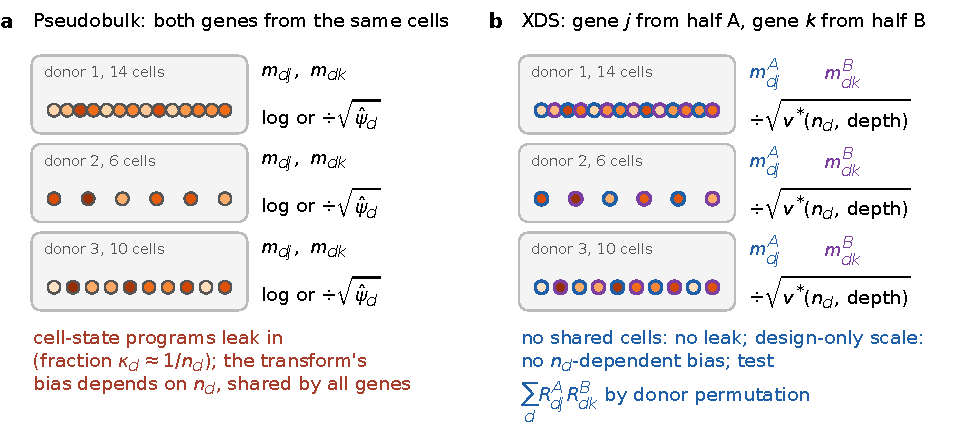
\includegraphics[width=\linewidth]{figures/fig_schematic.pdf}
\caption{Pseudobulk and XDS. Circles are cells; fill shade is a within-donor cell-state program. (a) Pseudobulk measures both genes on the same cells, so the program enters both donor means (the leak), and its log or self-standardized transform has an expectation that depends on the donor's cell number. (b) XDS measures gene $j$ on a random half of each donor's cells (blue outline) and gene $k$ on the other half (purple), and scales each mean by a variance that depends only on the donor's cell number and depths.}
\label{fig:schematic}
\end{figure}

\begin{theorem}[Validity of XDS with bounded cell numbers]\label{thm:xds}
Assume donors are independent; cells within a donor are i.i.d.\ given the donor's state, with depth independent of cell state; donor states are independent of designs; and $H_0$ holds. Treat $\mu$, $\sigma^2$, $\tau^2$ as known. Then for every donor and every $n_d\ge4$, $R^A_{dj}$ and $R^B_{dk}$ are independent given $Z_d$ and $\E[R^A_{dj}\mid Z_d]=0$, so $\E T_{jk}=0$ exactly and $\Var T_{jk}=\sum_d\E[(R^A_{dj})^2\mid Z_d]\,\E[(R^B_{dk})^2\mid Z_d]$. If in addition $n_d$ is bounded, the standardized counts have bounded $4+\delta$ moments, and $\psi^{*}$ is correctly specified, the permutation-moment statistic converges to $N(0,1)$ as $D\to\infty$. With the pooled plug-in estimates the same limit holds.
\end{theorem}

The contrast with leak correction is the point of the construction. A leak-corrected statistic is unbiased only if the per-donor leak estimate is, and its variance matches the permutation variance only if the leak estimate's own variance is negligible, which requires $\min_d n_d\to\infty$. XDS has no within-donor term to estimate: the leak (Proposition~\ref{prop:leak}) is zero because the two genes are measured on disjoint cells; the transformation bias (Proposition~\ref{prop:transform}) is zero because the standardization is design-only; and depth--state coupling enters only through $\E[m^h_{dj}\mid Z_d]$, which is unaffected when coupling does not vary systematically between donors. The price is that each gene uses half of each donor's cells, which costs power when donors are few and cells per donor are few (Section~\ref{sec:sim}).

\section{Results}\label{sec:results}

\paragraph{Data.} PsychAD frozen prefrontal-cortex microglia and perivascular macrophages (CELLxGENE dataset 09642770, \NnucPsy{} nuclei, 1,469 donors, 10x 3$'$ v3) \citep{Lee2023PsychADmyeloid}: subtypes Homeo\_CECR2 (\DPone{} donors with $\ge$4 nuclei, median \MedPone), PVM\_CD163 (\DPtwo, median \MedPtwo) and ADAM\_GPNMB (\DPthree, median \MedPthree). SEA-AD middle temporal gyrus microglia \citep{Gabitto2024SEAAD}: supertypes Micro-PVM\_1 (79 donors, median 15 nuclei) and Micro-PVM\_3 (83 donors, median 43). For each subtype we test all pairs among the 400 most expressed genes plus control genes not already among them (heat-shock, sex-linked and perivascular markers; 420--424 genes, about 89,000 pairs per subtype). Multiple testing uses Benjamini--Hochberg (BH) at $q=0.05$.

\paragraph{Comparators.} PB: Pearson correlation of log-CPM donor means. LCP: leak-corrected, self-standardized donor permutation (Appendix~\ref{app:methods}). The variants in Section~\ref{sec:neg} isolate each bias.

\subsection{Simulations with exact truth}\label{sec:sim}

The simulator draws latent donor and within-donor programs for 80 genes on the count scale (Appendix~\ref{app:sim}); true pairs have $\SB\neq0$ and nulls include pairs with only within-donor co-expression. Table~\ref{tab:sim} reports FDR and power. In large cohorts with a median of 20 cells per donor, pseudobulk's FDR rises from \LPBFDRa{} at 200 donors to \LPBFDRc{} at 1,000, and LCP's from \LLCPFDRa{} to \LLCPFDRc{}, as Theorem~\ref{thm:growth} predicts, whereas XDS stays at \LXDSFDRrange{} with power \LXDSpowRange. Theorem~\ref{thm:xds} assumes that depth is independent of cell state. In the same large designs with strong depth--state coupling (the stress setting of Appendix~\ref{app:sim}; frozen plan COUPLE\_PREREG), XDS had FDR \CoupleXDS{} at 200, 500 and 1,000 donors, whereas the U-statistic test XU, whose coupling bias is first order (Proposition~\ref{prop:coupling}), rose to \CoupleXU{}, LCP to \CoupleLCP{} and pseudobulk to \CouplePB{}. In small cohorts XDS remains calibrated (FDR \SXDSFDRrange{} in six designs with 16--83 donors) but loses power (\SXDSpowDforty{} versus \SLCPpowDforty{} for LCP at 40 donors with about 40 cells).

\begin{table}[t]\centering\small\setlength{\tabcolsep}{4pt}\caption{Simulations with exact truth. FDR (MCSE) at BH $q=0.05$ and power. $R=100$ replicates for designs with up to 83 donors, $R=50$ for larger designs. Pseudobulk and LCP lose FDR control as donors are added; XDS keeps it, and its power deficit disappears from about 500 donors.}\label{tab:sim}
\begin{tabular}{lcccccc}\toprule & \multicolumn{3}{c}{FDR} & \multicolumn{3}{c}{Power}\\\cmidrule(lr){2-4}\cmidrule(lr){5-7}
Design & PB & LCP & XDS & PB & LCP & XDS\\\midrule
16 donors, $\sim$40 cells & 0.216\,(0.022) & 0.110\,(0.025) & 0.025\,(0.013) & 0.047 & 0.014 & 0.002 \\
24 donors, $\sim$40 cells & 0.174\,(0.013) & 0.050\,(0.007) & 0.043\,(0.018) & 0.181 & 0.122 & 0.018 \\
40 donors, $\sim$40 cells & 0.133\,(0.006) & 0.051\,(0.004) & 0.041\,(0.006) & 0.499 & 0.501 & 0.156 \\
79 donors, Micro-PVM\_1 cells (median 15) & 0.594\,(0.011) & 0.077\,(0.004) & 0.041\,(0.007) & 0.321 & 0.399 & 0.070 \\
83 donors, Micro-PVM\_3 cells (median 43) & 0.179\,(0.006) & 0.051\,(0.002) & 0.048\,(0.003) & 0.877 & 0.929 & 0.665 \\
16 donors, $\sim$100 cells & 0.122\,(0.009) & 0.039\,(0.008) & 0.049\,(0.014) & 0.190 & 0.087 & 0.031 \\
200 donors, median 20 cells & 0.480\,(0.017) & 0.087\,(0.004) & 0.044\,(0.003) & 0.871 & 0.975 & 0.778 \\
500 donors, median 20 cells & 0.569\,(0.011) & 0.135\,(0.006) & 0.042\,(0.003) & 0.993 & 1.000 & 0.986 \\
1,000 donors, median 20 cells & 0.662\,(0.008) & 0.217\,(0.006) & 0.053\,(0.003) & 1.000 & 1.000 & 0.999 \\
\bottomrule\end{tabular}\end{table}


\subsection{Real-cell nulls: false discoveries grow with the number of donors}\label{sec:null}

Figure~\ref{fig:growth} and Table~\ref{tab:null} show the PsychAD pseudo-donor null. At full cohort size pseudobulk made \PBnullCalls{} false calls per reassignment (per-pair type-I error \PBnullTI), of which \PBrepFalse{} replicated (same sign, $p<0.05$) in an independent half of the pseudo-donors. LCP made \LCPnullCalls{} (type-I \LCPnullTI). XDS made at most one per reassignment, with type-I \XDSnullTI{} and \XDSnullTop{} for the 1\% of pairs with the strongest within-donor correlation, and no false call replicated. Pseudobulk's false calls rose from \PBgrowA{} at 25 pseudo-donors and \PBgrowC{} at 200 to the full-cohort totals; LCP made essentially none at 100 or fewer (\LCPgrowB) and thousands at full size. On three further reassignments drawn for a later plan, XDS again made a mean of \XDSfreshCalls{} false calls. In SEA-AD, with 79 and 83 pseudo-donors, XDS made no false calls and had type-I \SeaXDSTI{} (top 1\%: \SeaXDSTop), whereas LCP's top-1\% type-I was \SeaLCPTop{} and pseudobulk made \SeaPBcalls{} false calls per reassignment.

\begin{figure}[t]
\centering
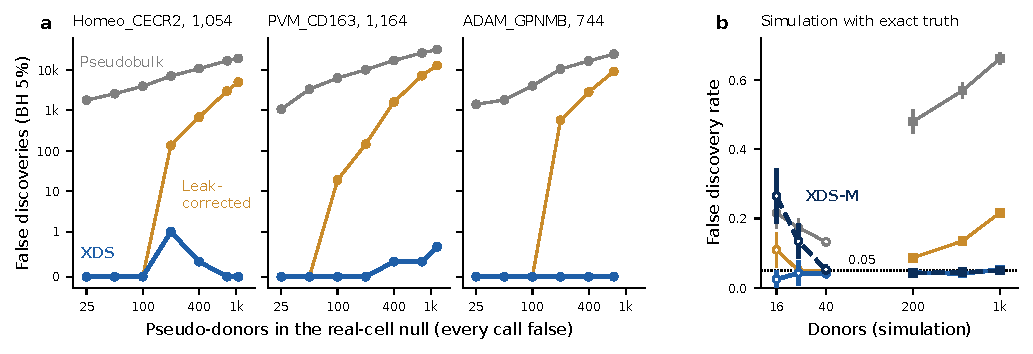
\includegraphics[width=\linewidth]{figures/fig_growth.pdf}
\caption{False discoveries grow with cohort size. (a) Mean BH false calls in the PsychAD real-cell null against the number of pseudo-donors (nested random subsets; three reassignments for 200 or more pseudo-donors, one for 25--100), for three myeloid subtypes; the panel title gives the full number of pseudo-donors. Every call is false. The vertical axis is linear below 1 and logarithmic above. (b) FDR in simulations with exact truth; open circles, about 40 cells per donor ($R=100$); filled squares, median 20 cells ($R=50$); bars, $\pm2$ MCSE. Pseudobulk and the leak-corrected test (LCP) degrade as donors are added; XDS does not.}
\label{fig:growth}
\end{figure}

\begin{table}[t]\centering\small\setlength{\tabcolsep}{3.5pt}\caption{PsychAD real-cell null at full cohort size (pseudo-donors; median nuclei), mean over three reassignments. Calls: BH false discoveries among $\sim$89{,}000 pairs. TI: per-pair type-I error at 0.05, over all pairs and over the 1\% most within-correlated pairs. Rep.: false calls replicated (same sign, $p<0.05$) in an independent half of the pseudo-donors.}\label{tab:null}
\begin{tabular}{lccccccccccc}\toprule & \multicolumn{3}{c}{PB} & \multicolumn{3}{c}{LCP} & \multicolumn{3}{c}{XDS} & \multicolumn{2}{c}{Rep.}\\\cmidrule(lr){2-4}\cmidrule(lr){5-7}\cmidrule(lr){8-10}\cmidrule(lr){11-12}
 Subtype & Calls & TI & top 1\% & Calls & TI & top 1\% & Calls & TI & top 1\% & PB & XDS\\\midrule
Homeo\_CECR2 (1{,}054; 28) & 19{,}158 & 0.335 & 0.920 & 4{,}986 & 0.201 & 0.360 & 0 & 0.050 & 0.053 & 3{,}876 & 0 \\
PVM\_CD163 (1{,}164; 19) & 31{,}617 & 0.441 & 0.919 & 12{,}880 & 0.301 & 0.705 & 1 & 0.050 & 0.051 & 12{,}515 & 0 \\
ADAM\_GPNMB (744; 12) & 24{,}544 & 0.378 & 0.979 & 9{,}125 & 0.265 & 0.787 & 0 & 0.048 & 0.047 & 7{,}876 & 0 \\
\bottomrule\end{tabular}\end{table}


The pseudo-donor null pools real donors, so real between-donor covariance becomes within-pseudo-donor covariance and the null's within-donor structure is somewhat stronger than that of real donors. The simulations, which have no pooling, show the same growth (Table~\ref{tab:sim}).

\subsection{What fails and why}\label{sec:neg}

Each correction we tried removes some biases and not others, and the ones it leaves are those Propositions~\ref{prop:leak}--\ref{prop:coupling} predict (Table~\ref{tab:ablate}). Removing the log transform (PBlin) leaves the leak. Leak subtraction with self-standardization (LCP) leaves the transformation bias and the error of the leak estimate; adding a jackknife variance for that error (LCP2) restored simulated FDR control but not the real-cell null. Design-only standardization with leak subtraction (LCPd) fixes the transformation bias but not the leak-estimate error, which matters most in the subtype with the fewest nuclei. Cross-splitting with self-standardization (LCPX) removes the leak but not the transformation bias, and with half of the cells per mean that bias is larger, so it made more false calls than LCP. An exact U-statistic with design weights and a studentized test (XU) removes the leak in expectation under independent depth, but depth--state coupling (Proposition~\ref{prop:coupling}) left \XUnullCalls{} false calls. Only the combination of disjoint cells and design-only standardization removes all three.

\begin{table}[t]\centering\small\setlength{\tabcolsep}{3pt}\caption{Each correction and the bias it leaves. Calls and TI: PsychAD real-cell null at full size (range over subtypes; XU on fresh reassignments). SEA-AD: type-I for the 1\% most within-correlated pairs in the SEA-AD real-cell null (79 and 83 pseudo-donors). LCP2 (not shown) had SEA-AD top-1\% type-I 0.068--0.085.}\label{tab:ablate}
\resizebox{\linewidth}{!}{\begin{tabular}{lllllll}\toprule Method & Standardization & Leak handling & Bias left & Calls & TI & SEA-AD\\\midrule
PB & log-CPM, own cells & -- & leak, transform & 19{,}158--31{,}617 & 0.335--0.441 & 0.607--0.674 \\
PBlin & ratio mean, own cells & -- & leak & 12{,}016--29{,}440 & 0.270--0.419 & 0.621--0.711 \\
LCP & self-standardized & subtract estimate & transform, leak-estimate error & 4{,}986--12{,}880 & 0.201--0.301 & 0.092--0.099 \\
LCPd & design-only & subtract estimate & leak-estimate error & 38--1{,}218 & 0.058--0.118 & 0.141--0.197 \\
LCPX & self-standardized & disjoint halves & transform (larger) & 15{,}538--32{,}801 & 0.354--0.497 & 0.074--0.153 \\
XU & design-only weights & exact U-statistic & depth--state coupling & 12{,}073--19{,}934 & 0.271--0.360 & 0.102--0.119 \\
XDS & design-only & disjoint halves & none detected & 0--1 & 0.048--0.050 & 0.043--0.050 \\
\bottomrule\end{tabular}}\end{table}


\subsection{False differential co-expression between Alzheimer's cases and controls}\label{sec:dc}

\DCtext{} In Homeo\_CECR2 the 816 XDS calls involve 215 genes, and the homeostatic receptors \emph{CX3CR1} and \emph{P2RY12} are the fifth and sixth most connected genes (post hoc, descriptive).

\subsection{Real donors}\label{sec:real}

On real PsychAD donors, between-donor co-expression is dense: XDS called \RealXDSfrac{} of pairs in the three subtypes, and \RealXDSrep{} of its calls in one random half of the donors replicated in the other half (pseudobulk: \RealPBrep). Pseudobulk made \RealPBonly{} calls per subtype that XDS did not. These are disagreements rather than proven errors, since XDS has less power, but the null results show that pseudobulk would make a comparable number of calls with no between-donor covariance at all.

\section{Discussion}\label{sec:disc}

The message for practice is that the donor being the unit of replication is necessary but not sufficient for valid between-donor co-expression. A per-donor summary must have an expectation that does not depend on the donor's cell number, and the two genes of a pair must not be measured on the same cells. Pseudobulk correlation violates both, and the violation is invisible at the cohort sizes on which it was validated. XDS satisfies both at a cost of power that disappears in large cohorts. For cohorts below about 100 donors, where XDS is underpowered, LCP is calibrated in simulation from 24 donors with about 40 cells per donor but exceeds nominal per-pair error for the most within-correlated pairs on real cells; we would report its results with that caveat.

\paragraph{Limitations.} The real-cell null pools donors (Section~\ref{sec:null}). XDS tests independence of donor effects, not zero covariance, and relies on depth--state coupling not varying systematically between donors; both are assumptions about real data that our nulls probe but cannot prove. One random split makes results depend on the split seed (Appendix~\ref{app:split}). We studied the 400 most expressed genes in myeloid cells of two brain cohorts; low-expressed genes and other tissues remain to be tested. The design-only standardization was introduced after an exploratory look at one pseudo-donor reassignment, which is excluded from every evaluation; all other analyses followed frozen plans.

\paragraph{Code and data availability.} Code, frozen plans with SHA-256 hashes, and all result files: [public repository URL]. Data are public on CZ CELLxGENE Discover.

\bibliographystyle{abbrvnat}
\bibliography{refs}

\clearpage
\appendix
\section{Proofs}\label{app:proofs}

\paragraph{Proposition~\ref{prop:leak}.} Write $m_{dj}=\sum_c (s_c/S_d)\,(Y_{cj}/s_c)$. Given $Z_d$ and the donor's state, cells are independent, $\E[Y_{cj}/s_c\mid\cdot]=\theta_{dj}$, and for $j\neq k$ the covariance of $Y_{cj}/s_c$ and $Y_{ck}/s_c$ within a cell equals $\SW_{d,jk}$ because measurement is conditionally independent across genes. Hence $\Cov(m_{dj},m_{dk}\mid Z_d,\text{state})=\sum_c(s_c/S_d)^2\SW_{d,jk}=\kappa_d\SW_{d,jk}$, and the law of total covariance over donor states (independent of $Z_d$) gives $\SB_{jk}+\kappa_d\bar\Sigma^{\mathrm W}_{jk}$. For independent donors whose ratio means share the expectation $\E\theta_{dj}$, $\E\sum_d(m_{dj}-\bar m_j)(m_{dk}-\bar m_k)=(1-\tfrac1D)\sum_d\Cov(m_{dj},m_{dk})=(1-\tfrac1D)\big(D\,\SB_{jk}+\sum_d\kappa_d\bar\Sigma^{\mathrm W}_{jk}\big)$; dividing by $D-1$ gives the claim with $\bar\kappa=D^{-1}\sum_d\kappa_d$. $\square$

\paragraph{Proposition~\ref{prop:transform}.} Under $H_0$, $g_{dj}$ and $g_{dk}$ are independent given $Z_d$, so $\E[g_{dj}g_{dk}]=\E\{\E[g_{dj}\mid Z_d]\E[g_{dk}\mid Z_d]\}$ and $\Cov(g_{dj},g_{dk})=\Cov_Z(b_j,b_k)$; centring at $\bar g$ costs $O(1)$ as in the previous proof. For $g=\log(1+am)$, a second-order Taylor expansion about $\theta_j$ gives $\E[g\mid Z]=\log(1+a\theta_j)-\tfrac{a^2}{2}\Var(m\mid Z)/(1+a\theta_j)^2+O(\E|m-\theta|^3)$, and $\Var(m_{dj}\mid Z_d)=\SB_{jj}+\kappa_d\bar\Sigma^{\mathrm W}_{jj}+\theta_j/S_d$ depends on $n_d$ through $\kappa_d$ and $S_d$. For $g=(m-\mu)(\tau^2+\hat\psi)^{-1/2}$, expanding $(\tau^2+\hat\psi)^{-1/2}$ about $\tau^2+\psi$ gives $\E[g\mid Z]=-\tfrac12(\tau^2+\psi)^{-3/2}\Cov(m,\hat\psi\mid Z)+O(\E|\hat\psi-\psi|^2)$, and $\hat\psi_{dj}=\kappa_d\hat\sigma^2_{dj}+m_{dj}/S_d$ is positively correlated with $m_{dj}$ (through $m_{dj}/S_d$ and the mean--variance relation of $\hat\sigma^2$), with a covariance that shrinks as $n_d$ grows. $\square$

\paragraph{Proposition~\ref{prop:coupling}.} Let $a_c=s_cf_j(s_c)$ and $b_c=s_cf_k(s_c)$. Given $Z_d$ and the donor's state, $\E[Y_{cj}]=a_c$, $\E[Y_{ck}]=b_c$, and cells are independent, so $\E\sum_{c\neq c'}Y_{cj}Y_{c'k}=\sum_{c\neq c'}a_cb_{c'}=(\sum a)(\sum b)-\sum_c a_cb_c$. With $Q_d=\sum_cs_c^2$,
\begin{align*}
\E[u_{djk}]-\E[m_{dj}]\E[m_{dk}]&=\frac{(\sum a)(\sum b)-\sum a b}{S_d^2-Q_d}-\frac{(\sum a)(\sum b)}{S_d^2}\\
&=-\frac{Q_d}{S_d^2-Q_d}\Big[\sum_c w_cf_j(s_c)f_k(s_c)-\Big(\sum_cv_cf_j(s_c)\Big)\Big(\sum_cv_cf_k(s_c)\Big)\Big],
\end{align*}
with $w_c=s_c^2/Q_d$ and $v_c=s_c/S_d$. The bracket vanishes when $f_j,f_k$ are constant in $s$ and is first order in the depth slopes of $f$ otherwise, because the two weightings have different means of $s$. This is the exact form of the statement in the main text. $\square$

\paragraph{Theorem~\ref{thm:growth}.} $(T_D-\sum_d\beta_d)/\sqrt{\sum_d\Var h_d}\Rightarrow N(0,1)$ by Lindeberg's theorem (bounded variances; we assume uniformly bounded $2+\delta$ moments). If $\frac1D\sum\beta_d\to\bar\beta\neq0$, then $|\sum_d\beta_d|/\sqrt{\sum_d\Var h_d}\ge|\bar\beta|\sqrt{D/\bar v}\,(1+o(1))\to\infty$, so $|T_D|/\hat\sigma_D\to\infty$ in probability. If $\sum_d\beta_d=o(\sqrt D)$ the centring is asymptotically negligible and the rejection probability tends to $\alpha$. $\square$

\paragraph{Theorem~\ref{thm:xds}.} Given $Z_d$ and the donor's state, the cells in $A_d$ and $B_d$ are independent, and the split is independent of the data. $R^A_{dj}$ is a function of the gene-$j$ data in $A_d$ and of $Z_d$ (through $\psi^{*}$), and $R^B_{dk}$ of the gene-$k$ data in $B_d$ and $Z_d$. Under $H_0$ the donor-level quantities for $j$ and $k$ are independent given $Z_d$, so $R^A_{dj}\perp R^B_{dk}\mid Z_d$. With depth independent of state, $\E[m^A_{dj}\mid Z_d,\text{state}]=\theta_{dj}$, hence $\E[m^A_{dj}\mid Z_d]=\E\theta_{dj}=\mu_j$ because states are independent of designs, and $\E[R^A_{dj}\mid Z_d]=0$; this uses no property of $n_d$ other than $|A_d|,|B_d|\ge2$. Independence across donors gives $\E T=0$ and the stated variance. Under (A5), $\E[(R^A_{dj})^2\mid Z_d]=c_j$ and $\E[(R^B_{dk})^2\mid Z_d]=c_k$ for all donors, so $\Var T=Dc_jc_k$. The permutation mean is $D\bar R^A_j\bar R^B_k=O_p(1)$, and the permutation variance $(D-1)^{-1}\sum_d(R^A_{dj}-\bar R^A_j)^2\sum_d(R^B_{dk}-\bar R^B_k)^2=Dc_jc_k(1+o_p(1))$ by the law of large numbers; Lindeberg's theorem for $\sum_dR^A_{dj}R^B_{dk}$ with bounded $2+\delta/2$ moments (implied by bounded $4+\delta$ moments of each factor) gives the limit. Replacing $\mu,\sigma^2,\tau^2$ by pooled estimates perturbs each $R_{dj}$ by a common $O_p(D^{-1/2})$ term per gene; the induced change in $T/\sqrt D$ is $O_p(D^{-1/2})$ times sample means of $R$, which are $O_p(D^{-1/2})$, so it is $o_p(1)$ for each pair (Slutsky). This is a pairwise statement; uniformity over all pairs, which BH would need, is not shown. $\square$

\section{Methods compared}\label{app:methods}

All methods use the donor ratio means $m_{dj}$, the model-based sampling variance $\hat\psi_{dj}=\kappa_d\hat\sigma^2_{dj}+m_{dj}/S_d$ with $\hat\sigma^2_{dj}$ the donor's own Poisson-corrected within-cell variance, and Paule--Mandel estimates $\hat\mu_j,\hat\tau^2_j$.
\begin{itemize}\itemsep0pt
\item \textbf{PB}: Pearson correlation of $\log(1+10^6m_{dj})$ across donors, Fisher $z$ test. \textbf{PBlin}: the same without the log.
\item \textbf{LCP}: $r_{dj}=(m_{dj}-\hat\mu_j)/(\hat\tau_j^2+\hat\psi_{dj})^{1/2}$; $T=[\sum_d(r_{dj}r_{dk}-\tilde\ell_d)]\sqrt{D/(D+\sum_d\tilde\ell_d^2)}$ with leak estimate $\tilde\ell_d=\kappa_d\hat C_{d,jk}/(\hat v_{dj}\hat v_{dk})^{1/2}$; donor-permutation reference. \textbf{LCP2} adds a delete-one-cell jackknife estimate of the leak estimate's variance to the scaling factor.
\item \textbf{LCPd}: LCP with design-only $\psi^*$ in place of $\hat\psi$. \textbf{LCPX}: cross-split with self-standardization in each half. \textbf{XDS}: cross-split with design-only standardization (Section~\ref{sec:xds}).
\item \textbf{XDS-M}: $S=5$ independent splits per donor (the first is the XDS split); $q_d$ is the mean over splits of $R^{A_s}_{dj}R^{B_s}_{dk}$; one-sample $t$ test with normal reference. \textbf{KX}: per-donor products $y_d=R^*_{dj}R^*_{dk}$ with full-donor design-only standardization, regressed on $x_d=\kappa_d(v^*_{dj}v^*_{dk})^{-1/2}$ by least squares; the intercept is tested with a heteroscedasticity-robust (HC0) standard error.
\item \textbf{XU}: $q_d=w_d(u_{djk}-c_{dk}m_{dj}-c_{dj}m_{dk}+c_{dj}c_{dk})$ with $u$ the off-diagonal U-statistic, $c$ a leave-one-donor-out mean and design-only weights $w_d=(v^*_{dj}v^*_{dk})^{-1/2}$; one-sample $t$ test on $(q_d)_d$.
\end{itemize}
\textbf{Donor-centred null.} For each real donor and gene, the Paule--Mandel shrunken donor effect $\tilde\theta_{dj}=\mu_j+\tau_j^2(\tau_j^2+\hat\psi_{dj})^{-1}(m_{dj}-\mu_j)$ defines a factor $f_{dj}=\mu_j/\tilde\theta_{dj}$ (clipped to $[0.1,10]$); every count of the donor's cells is multiplied by $f_{dj}$ before pooling and reassignment. This removes most between-donor differences while keeping within-donor structure. Permutation $p$-values use $10^5$ shared donor permutations when $D\le100$; for $D\ge200$ we use the normal approximation with the exact permutation mean and variance. Runtime for XDS on 1,164 donors and 87,990 pairs is under one minute on one laptop CPU core.

\section{Simulator}\label{app:sim}

The simulator has exact analytic truth on the latent scale. Each 80-gene panel (3,160 pairs) contains within-only programs (moderate and strong), between-only programs, programs at both levels with the same and opposite signs, a sign-heterogeneous within-donor null, a between-donor weak null (dependent but uncorrelated donor effects) and independent genes. Donor effects are log-normal with gene-specific donor variation matched to SEA-AD; per-cell depths follow the SEA-AD fit. All results use the held-out panel (seed 4112026), which was not used to develop any method. Small designs: 16, 24 and 40 donors with about 40 cells; 16 donors with about 100 cells; the exact cell numbers of SEA-AD Micro-PVM\_1 and Micro-PVM\_3 ($R=100$). Large designs: 200, 500 and 1,000 donors with a median of 20 cells ($R=50$). Coupling stress designs add a depth--state coupling in which each cell's depth is multiplied by $\exp(0.3\,z)$, with $z$ its within-donor program score, and the standard deviation of residual log depth is doubled ($R=50$). FDR is the mean false discovery proportion over replicates; power is the mean fraction of true pairs called; MCSEs are given in the tables.

\section{Split-seed dependence}\label{app:split}

\SplitText

\section{Analysis plans, amendments and outcomes}\label{app:prereg}

Each plan was written and hashed (SHA-256) before the computations it governs; files are in \texttt{prereg/} of the repository.
\begin{itemize}\itemsep0pt
\item \textbf{FIX\_PREREG} (real-cell null in SEA-AD; LCP2). Outcome: pseudobulk false discoveries in real cells YES; LCP and LCP2 fail the top-1\% criterion; LCP2 not adopted (power 0.87 of LCP's at 24 donors).
\item \textbf{XS\_PREREG} (LCPX). Amendment before any full run: the weak null is the class QQ\_cross only. Outcome: negative on all three criteria.
\item \textbf{POP\_PREREG} (PsychAD). Outcomes: false discoveries grow with cohort size YES in all subtypes; replication does not protect pseudobulk YES; LCPX holds at population scale NO. Deviation: the $D\le100$ points were run after the larger ones and for one reassignment per subtype.
\item \textbf{DSTD\_PREREG} (LCPd, XDS). Written after one exploratory reassignment (excluded). Outcomes: LCPd not adopted (fails the SEA-AD null); XDS holds every null but fails the frozen power criterion against LCP at 24 and 40 donors, so by that rule it does not replace LCP in small cohorts; the frozen claim comparing LCP with LCPd failed (LCPd type-I 0.058--0.118 at full size); the analogous LCPX-versus-XDS contrast is given in Table~\ref{tab:ablate} as a post hoc comparison.
\item \textbf{XU\_PREREG} (XU). Outcome: XU fails the population-scale real-cell null; XDS remains the recommended large-cohort test.
\item \textbf{COUPLE\_PREREG} (coupling stress, no decision). Outcome as predicted: XDS close to nominal, XU, LCP and pseudobulk inflated and growing with $D$.
\item \textbf{DC\_PREREG} (AD differential co-expression). Outcomes in Section~\ref{sec:dc}.
\item \textbf{REV\_PREREG} (written after an internal review, before its computations): run-level error in 100 reassignments per subtype; XDS-M and KX; group-centred XDS-DC; positive control; size of false edges; amendment R6 (donor-centred null) added before R6 was computed. Outcomes: single-split XDS with the normal reference fails the run-level criterion; XDS-M passes; KX fails in one subtype.
\item \textbf{ONEK\_PREREG} (OneK1K). Amendment before any test: genes ranked on a 5,000-cell subsample; XDS-M added.
\end{itemize}
The split-seed analysis (Appendix~\ref{app:split}) and the sign analysis of pseudobulk false calls were post hoc.

\end{document}
